\documentclass[a4paper,12pt]{book}

% Packages
\usepackage{geometry}          % Page dimensions
\usepackage{fancyhdr}          % Custom headers and footers
\usepackage{hyperref}          % Hyperlinks
\usepackage{amsmath, amssymb}  % Math symbols
\usepackage{listings}          % Code listings
\usepackage{xcolor}            % Color support
\usepackage{graphicx}          % Include graphics
\usepackage{tikz}              % For diagrams
\usepackage{imakeidx}          % Index
\usepackage{glossaries}        % Glossary
\usepackage{titlesec}          % Custom titles for chapters

% Setup page margins
\geometry{a4paper, margin=1in}

% Custom header and footer
\pagestyle{fancy}
\fancyhf{}
\fancyhead[L]{\leftmark}   
\fancyhead[R]{\thepage}    

% Listings configuration for code
\lstset{
  language=Java,
  basicstyle=\ttfamily\footnotesize,
  keywordstyle=\color{blue},
  stringstyle=\color{red},
  commentstyle=\color{green!70!black},
  numbers=left,
  numberstyle=\tiny\color{gray},
  frame=single,
  breaklines=true
}

% Redefine chapter format (remove chapter number, center the title)
\titleformat{\chapter}[display]
  {\normalfont\huge\bfseries\centering} % Chapter title format: large, bold, centered
  {} % No chapter number
  {20pt} % Space between the number and the title
  {\Huge} % Title format: large
  []

% Title and TOC
\title{Your Book Title}
\author{Your Name}
\date{\today}

\makeglossaries
\makeindex

\begin{document}

\maketitle
\tableofcontents
\newpage

% Chapter 1: Introduction
\chapter{Introduction}
This chapter introduces the main topics of the book.

\section{Purpose}
The purpose of this book is to...

\section{Structure}
The book is organized into chapters...
% Chapter 2: Images and Code Examples
\chapter{Images and Code Examples}
This chapter covers how to include images and code examples.

\section{Including Images}
You can include images as follows:

\begin{figure}[h]
  \centering
  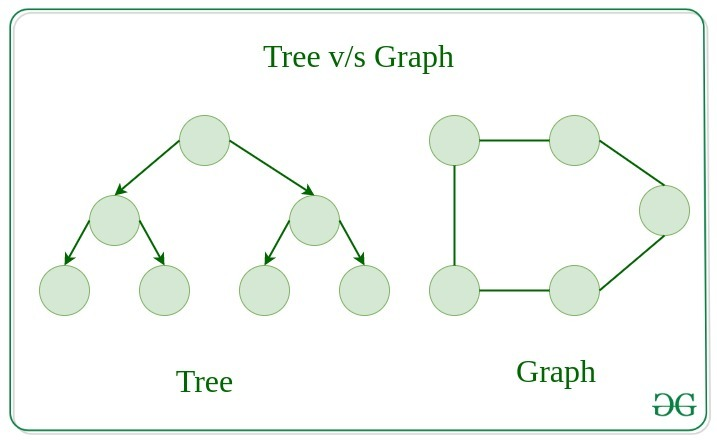
\includegraphics[width=0.5\textwidth]{images/tree_vs_graph.jpg}
  \caption{An example image.}
  \label{fig:example-image}
\end{figure}

\section{Java Code Example}
Here’s an example of a simple Java program:

\lstinputlisting[language=Java, caption=Hello World Program]{com/pol/Example.java}
% Chapter 3: Advanced Topics
\chapter{Advanced Topics}
This chapter discusses more advanced topics...

\end{document}
